\documentclass[11pt,a4paper,oneside,openany]{jsreport}
%
\usepackage[dvipdfmx]{graphicx}
%
\usepackage{comment}
\usepackage{tipa}
\usepackage{natbib}
\usepackage{url}
\usepackage{gb4e}
\usepackage{float}
\usepackage{ascmac}
\usepackage{pxrubrica}
\usepackage{remreset}

\makeatletter\@removefromreset{footnote}{chapter}\makeatother
\bibpunct[: ]{(}{)}{,}{a}{ }{,}
\renewcommand{\theenumi}{\alph{enumi}}
%
\newcounter{tempcnt}
\newcommand{\exn}[1]{%
\setcounter{tempcnt}{\value{exx}}%
\addtocounter{tempcnt}{#1}%
\arabic{tempcnt}}
%
\title{ソロモン諸島のピジン(Pijin)語における従属節標識について}
\author{栗田健太郎}

\begin{document}
\maketitle
% \begin{abstract}
% ソロモン諸島の\ruby[g]{共通言語}{リンガ・フランカ}であるPijin語は、英語を主な語彙供給源とするメラネシア・ピジンの1つであるが、包括的な文法書は未だに発行されておらず、公用語としての地位もないため、地域や時代による変化が激しいとされる。本論文では、現在のPijin語の文法に迫る1つの試みとして、\textit{dat}、\textit{fo}の従属節標識としての用法を、近年発行されたPijin語の聖書についてのコーパス分析と、ソロモン諸島の首都ホニアラでの容認度調査を元に示す。
% \end{abstract}

\tableofcontents
\chapter{序論}

% アブスト
%
% ソロモン諸島の\ruby[g]{共通言語}{リンガ・フランカ}でもあるPijin語は、英語を主な語彙供給源とするメラネシアン・ピジンの1つであるが、包括的な文法書は未だに発行されておらず、公用語としての地位もないため、地域や時代による変化が激しいとされる。本論文では、現在のPijin語の文法に迫る1つの試みとして、\textit{dat}、\textit{fo}の従属節標識としての用法を、近年発行されたPijin語の聖書についてのコーパス分析と、ソロモン諸島の首都ホニアラでの容認度調査を元に示す。

\section{Pijin語の概略}
\section{英語との関係}

\chapter{dat}

本章で取り扱う\textit{dat}は音韻的に英語の\textit{that}に由来することは明らかと言えそうだが、従来のほとんどの研究では限定詞\textit{datfala}や\textit{datwan}の語幹としての用法しか示されていなかった。本章では、この\textit{dat}が現代のPijin語の中で名詞節を作る従属節標識としての用法があることを示し、聖書の用例を検討・コーパス分析した上で、現地ホニアラでの簡易的な容認度調査の結果を紹介する。さらに、考察としてその発音や英語\textit{that}節の用法との比較、そして意味的に似た場面で用いられる\textit{olsem}の分布を紹介する。その結果、\textit{dat}は特定の動詞の後ろに来て、文中の働きとしては直接目的語にあたる名詞節を形成する用法でのみ使用されていることが明らかになる。

\section{従来の意味}

\textit{dat}は\cite{dictionary}中に\textit{dat}単体の形で語彙として挙げられていない一方で、\textit{datfala}「その」「それ(具体的)」、\textit{datwan}「それ」という形がそれぞれ別個の指示詞として掲載されている。(\exn{1})はその\textit{datfala}の項で挙げられている例文であり
\footnote{以下、特にことわりが無ければグロスは筆者。用いる略号は基本的に\cite{prepositions}に従ったが、いくつかの必要な略号は補った: 1/2/3=1st/2nd/3rd person, SG=singular, DU=dual, PL=plural, INC=inclusive, EXC=exclusive, DEIC=deictic, PM=predicate marker, FUT=future, PERF=perfective, NEG=negative, DAT=dative, LOC=locative, POSS=possessive, TOP=topic, STATM=statement}
、ここでは\textit{datfala}が前置の修飾語として用いられているのがわかる。

\begin{exe}
  \ex
  \gll Datfala tri ia, hem long lan blong mi ia.\\
  that tree DET 3SG LOC land POSS 1SG DET\\
  \glt `That tree is on my land.'
\end{exe}

\textit{-fala}は主として形容詞接辞、\textit{-wan}は形容詞や状態動詞を名詞に変える働きを持つ接辞である\footnote{この定義は\cite{syntax}に従った。\textit{-fala}の形が定着した単語においては、直前に見た\textit{datfala}の名詞用法、三人称双数代名詞としての\textit{tufala}、一人称複数代名詞としての\textit{mifala}のように、共時的には必ずしも形容詞接辞として解釈できない意味を持つ単語もある。}一方で、徐々に多くの話者から省略されるようになってきている\citep{syntax}。
そのため、\textit{dat}単独での形でも、「その」「それ」という代名詞や限定詞としての意味を持つと推測され、事実インフォーマントへの調査においても、特定の例文を示すことなく\textit{dat}のPijin語における語義を尋ねると、この限定詞としての意味を説明されることが多かった。

\section{名詞節を形成する従属節標識として}

しかし、これから\ref{sec:datbib}節で説明するように、Pijin語聖書の中には\textit{dat}がそのままの形で現れる例が非常に多く、その意味は明らかに限定詞\textit{datfala}, \textit{datwan}の短縮形として解釈できない。この\textit{dat}は直後に節として解釈できる名詞・動詞などの単語が続く場合が多く、結論としては英語の\textit{that}節のように従属節標識としての機能があると考えられる。

\subsection{聖書中の用法}\label{sec:datbib}
Pijin語の新約聖書においては、\textit{dat}は単独で頻繁に登場し、その用例は全て従属節標識として解釈できる。実際の例として(\exn{1})を挙げる。\textit{dat}の後には節主語として解釈できる\textit{olketa samting ia}「この事ごと」、Pijin語を含むメラネシア・ピジン特有の述語標識\textit{i}、そして節動詞として解釈できる\textit{hapen}「起こる」と続いていて、これらの節としての意味「この事々が実際に起こったということ」が文全体の述語\textit{save}「知る」の目的語となっていることが分かる。

\begin{exe}
\ex
\gll An yufala save \underline{dat} olketa samting ya i hapen tru nao.\\
and 2PL know \underline{that} PL thing DEIC PM happen truly PERF\\
\glt `And you all know that the things really happened.' (1TH 3:4)
\end{exe}

\textit{dat}の用例は673に上り、筆者の観察ではその全てが従属節標識としての使用であった。
\textit{dat}の直前の位置に来る単語の分布を表\ref{tb:datl1}に示す。

\begin{table}[h]
  \caption{datの直前の位置に来る単語(1~8位)}
  \label{tb:datl1}
  \begin{minipage}{0.5\hsize}
  \begin{center}
    \begin{tabular}{|c||c|l|} \hline
      単語 & 分布数 & 対応する意味 \\ \hline \hline
      save & 168 & know\\ \hline
      somaot & 87 & show\\ \hline
      lukim & 72 & look\\ \hline
      luksave & 49 & recognise\\ \hline
    \end{tabular}
  \end{center}
  \end{minipage}
  \begin{minipage}{0.5\hsize}
    \begin{center}
      \begin{tabular}{|c||c|l|} \hline
        単語 & 分布数 & 対応する意味 \\ \hline \hline
        herem & 41 & hear \\ \hline
        talemaot & 32 & announce, reveal\\ \hline
        nao & 28 & PERF\\ \hline
        talem & 28 & tell, say\\ \hline
      \end{tabular}
    \end{center}
  \end{minipage}
\end{table}

特筆すべきことは、\textit{dat}の直前に来る単語はほとんど全てが動詞だということである。Pijin語がわりと典型的なSVO型の言語であることからも、あるいは実際の用例の観察からも、動詞の直後に来る\textit{dat}節は(\exn{0})同様に文の目的語として機能していることが分かる。表\ref{tb:datl1}の7位を占める副詞\textit{nao}は唯一動詞ではないが、この表に集計されている文章ではその全てが動詞の直後に来て完了を示す用法で使われていた\footnote{\textit{nao}は多義的な単語であり、その位置によっては全く異なる文法的意味を持つ。名詞の直後に置いてその節の話題を示したり、節の先頭につけてその節の時間的な前後関係を示す用法、あるいは文の終わりを示す用法(cf.(\ref{ex:naostatm}))が辞書\citep[145]{dictionary}には示されている。}。そして、この28例の\textit{nao dat}という単語連続は、「動詞+\textit{nao}+\textit{dat}節」というように別の動詞と\textit{dat}節の間に\textit{nao}が挿入されただけであり、\textit{dat}節自体は別の動詞の目的語としての文法的機能を担っている。実際の例として(\exn{1})を示す。ここでの\textit{dat}節は他動詞\textit{luksave}「認識する、見て分かる」の目的語となっている。

\begin{exe}
\ex
\gll ...bae olketa luksave nao \underline{dat} man ya hemi tinghae long yu.\\
FUT 3PL recognise PERF \underline{that} man DIEC 3SG-PL respect LOC 2SG\\
\glt `...then they will recognise that the man respects you.' (LUK 14:11)
\end{exe}

%このような従属節標識としての\textit{dat}の使用は、これまでPijin語について書かれてきた文法概要\cite{syntax}や辞書\cite{dictionary}、さらに現地で発行されている入門書\cite{yumi}には記載が無い一方、\cite{eric}にはごく簡単にこの用法の解説がされていた。%

\subsection{現地調査}\label{sec:datfield}

これらの聖書中の用例を踏まえ、\ref{sec:howexamined}節に述べた方法で現地での容認度調査を行った。調査は筆者が作った(\exn{1})、(\exn{2})を元にして行った。

\begin{exe}
\ex\label{dat1}
\gll Hemi talem \underline{dat} yu stap long hia.\\
3SG-PM tell \underline{that} 2SG be at here\\
\glt `He told that you are here.'
\ex\label{dat2}
\gll Mi no save \underline{dat} hem nao draev.\\
1SG NEG know \underline{that} 3SG TOP drive\\
\glt `I didn't know that he will drive.'
\end{exe}

結果、全てのインフォーマントからこの文は適格であると認められた。意味の違いについて尋ねたところ、2つの文に違いがあると述べたインフォーマントはいなかった。若い話者のほとんどは自分で話すときにも\textit{dat}を用いることがあると述べた一方で、ある50代のインフォーマント\footnote{ガダルカナル島東部のAola村の出身で、母語はLengo(オーストロネシア語族、南東ソロモン諸語)。ホニアラに来てPijinを覚えたのは30年以上前だという。}は自分以上の年代では\textit{dat}単体での使用は違和感を感じるかもしれないと答え、次のような3通りの言い方なら許されただろうと述べた。\textit{bae}は未来を示すマーカーだがPijin語にはっきりとした時制はなく\citep{eric}、未来を示す文章でも必ずしも用いる必要はない\footnote{
  話者や文の構造による\textit{bae}(あるいは\textit{baebae}, \textit{bambae})の分布を詳細に調べた論文として\cite{bae}がある。
}。

\begin{exe}
\exi{(\exn{-1}$'$)} Hemi talem \underline{bae} yu stap long hia.
\exi{(\exn{-1}$''$)} Hemi talem \underline{dat} \underline{bae} yu stap long hia.
\exi{(\exn{-1}$'''$)} Hemi talem yu stap long hia.
\end{exe}

その後60代のインフォーマント\footnote{マライタ島南部出身で、母語はBaelelea(同じく南東ソロモン諸語)。Pijin語は第2言語として覚えたという。}に尋ねたが、彼女はこのような傾向を見せず、(\exn{-1})から(\exn{-1}$'''$)すべての文章が等しく正しいと答えた。その一方で、これらの文章はやや「宗教っぽい」響きがすると述べた。

\section{考察}
\subsection{発音}
前述した通り、\textit{dat}の従属節標識としての使用はほとんどの文法書や辞書には記載が無かったが、語学入門書である\cite{eric}には簡潔な記載がある\footnote{
\cite{eric}\vspace{0.1in}
\begin{quote}
\begin{exe}
  \exi{3.} Mi talem hem dat Bili hem i stap long Kukum. \\
  `I told him that Billy lives in Kukum.'
\end{exe}\vspace{0.1in}
Some verbs in Pijin can take \underline{\texttt{dat*}} + SENTENCE as an object instead of a simple noun phrase.
\begin{screen}
NOTE: *There are many areas in the Solomons where \underline{\texttt{dat}} is not used: Speakers who don't use \underline{\texttt{dat}} will say that the two clauses with an intonation that suggests that they are two independent sentences, or use a word borrowed from a local language.
\end{screen}
\end{quote}
}。30年以上前の記述ではあるが、この入門書によれば、本論で取り扱うような従属節標識としての用法で\textit{dat}が用いられない地域も多く、\textit{dat}を用いない話者は従属節を「2つの節が2つの独立した文であることを示すようなイントネーション」\footnote{上注の囲み部分参照。意味的にはむしろこの否定が正しいように思われるが、誤植だろうか。}によって、あるいは現地の言葉から借用した言葉によって話すと述べられている。

今回の都市部における調査では、そもそも\textit{dat}を許容しない話者を見つけられなかったため、後者の現地からの借用語については確認することができなかったが、前者のイントネーションについてはある程度確認できたため、非常に粗縛な形ではあるがここに分析する。\cite{eric}の記述によれば、通常の叙述文の一般的なイントネーションのパターンは図\ref{fig:intonation}のような形を取る。文は中間くらいの高さ(2)で比較的平坦に話され、文の最後となる強勢で上がり(3)、それから低く落ちる(1)。

\begin{figure}[ht]
  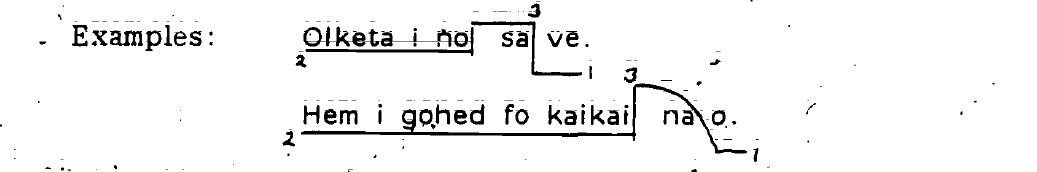
\includegraphics[width=15cm]{./intonation.png}
  \caption{Pijin語叙述文における一般的なイントネーションのパターン\cite[10]{eric}}
  \label{fig:intonation}
\end{figure}

今回筆者が録音した用例を聞く限りでは、\textit{dat}を用いずに動詞の目的語として節を取る発話では(a)速い発話では、動詞に続いて間を置かずに話される (b)ゆっくりの発話では、文が続くことを示すために動詞の語尾が下降しない という特徴があるように感じられた。いずれの場合においても、イントネーションは2つの節(主節、従属節)がバラバラの2つの文ではなく、全体で1つの文であるということを考えれば、図\ref{fig:intonation}のパターンに合致しているように思われる。通常文が終わるタイミングではイントネーションが下降するため、ゆっくりの発音でもその下降がなければ聞き手に一文がまだ続いているという情報を伝えることができる。しかし、このイントネーションが\cite{eric}によって示されたものと同一であるかどうかには疑念がある。

\cite{phonology}はPijin語についてのイントネーションに対する研究はほとんど無いと前置きした上で、イントネーションがPijin語の文の意味解釈に与える影響の大きさについて記している。その一方で将来のPijin語について、「ことによると文法化の進行は情報伝達におけるイントネーションの必要性を減少させるかもしれず、言語がより成熟しより標準化していく中で、ことによるとイントネーションの使用は文法的標識に役割を譲り、音韻はより標準的なものになるかもしれない」\footnote{``Perhaps increasing grammaticalization will reduce the need for intonation in conveying information and, as the language gets older and more standardized, perhaps the use of intonation will give way to grammatical markers, and the phonology will become more regular.''\citep{phonology}}とも述べている。\textit{dat}という従属節標識の(部分的な)導入とこの節で示したイントネーションとの関係は、まさにここで示されているような現象の1つかもしれない。

\subsection{英語のthat節との比較}\label{sec:vsthat}

ここで取り上げたような\textit{dat}の従属節標識としての使用は、その発音からも用法からも英語の\textit{that}節からある程度の影響があったということは否定できないだろう。一方で、これから検証していくように、少なくとも聖書の中での用法は英語と比較して限定的であり、借用はある程度限定的である。Pijin語と英語の文法を単純に比較することには問題があるかもしれないが、この節では一応の比較を試みてみる。

まず、英語の\textit{that}節には制限用法に限って関係節標識としての用法が存在する\cite[365--367]{english}が、Pijin語の\textit{dat}には見当たらない。\cite{dictionary}には関係節標識として\textit{we}と\textit{hu}が挙げられているが、聖書の場合も同様の用法で\textit{wea}と\textit{hu}を利用している。

さらに、名詞従属節標識としての機能も、英語に比べるとかなり限られている。\cite{english}は文中の英語\textit{that}節の用法として次の5つを挙げている。

\begin{enumerate}
  \item 主語 : \textit{That the invading troops have been withdrawn} has not affected our government's trade sanctions.
  \item 直接目的語 : I noticed \textit{that he spoke English with an Australian accent}.
  \item 主格補語 : My assumption is \textit{that interest rates will soon fall}.
  \item 同格 : Your criticism, \textit{that no account has been taken of psychological factors}, is fully justified.
  \item 形容詞補語 : We are glad \textit{that you are able to join us on our wedding anniversary}.
\end{enumerate}

Pijin語における\textit{dat}節の働きは、聖書で筆者が観察した限りでは(b)すなわち直接目的語としての用法に限られていて、それ以外の用法は別の従属節標識が担っているように思われる。すなわち、(c)(d)は次節で取り上げる\textit{olsem}が、(a)(e)は次章で取り上げる\textit{fo}が用いられているのである。

\subsection{olsem節}
\textit{olsem}は\cite{dictionary}では「~のような(like that, as if)」という意味のみが挙げられている。従属節標識としての例文は(\exn{1})が挙げられているが、ここでの\textit{olsem}節も同様の意味で解釈できる。
%
\begin{exe}
  \ex\label{ex:naostatm}
  \gll Man toktok \underline{olsem} hem bikman nao.\\
  man talk \underline{like} 3SG important-man STATM\\
  \glt ``This man talks as if he were an important man.'' \citep[157]{dictionary}
\end{exe}
%
しかし、前節で取り上げたように、聖書では(c)主格補語 (d)補語 として名詞的従属節を導入する際には\textit{dat}は用いられず、代わりに\textit{olsem}が使われる。
%例文見つからない%

\begin{exe}
  \ex\label{ex:olsemc}
  \gll Mining blong disfala toktok ya hemi \underline{olsem} hemi haed from olketa, ...\\
  meaning POSS this story DEIC 3SG-PM \underline{like} 3SG-PM \\
  \glt ``This man talks as if he were an important man.'' (LUK 18:34)
\end{exe}

また、聖書では引用符つきで登場人物の発言を引用する、いわゆる直接話法のような形式で台詞が挿入されることも多い。その場合、必ずしも義務的ではないものの、\textit{olsem}がよく括弧の直前に発言を示す標識として導入される。(\exn{1})(\exn{2})はその例である。

\begin{exe}
  \ex
  \gll Nao olketa tok \underline{olsem}, ``Bat bos, hemi garem plande finis ya."\\
  TOP 3PL say \underline{like} but boss 3SG-PM have many PERF DIEC\\
  \glt They said, ``But boss, he already have many (money)."(LUK 19:25)

  \ex\label{ex:talemolsem}
  \gll Buktambu hemi talem klia \underline{olsem}, ``Bae tufala kamap wanfala bodi nomoa." \\
  book-holy 3SG-PM say clearly \underline{like} FUT 3DU appear one body only\\
  \glt ``The holy book says clearly, `the two will become one flesh.'"(1CO 6:16)
\end{exe}

\textit{olsem}には従属節標識以外にも様々な用法があり、今回行った単純な集計には前置詞としての用法等も含まれてしまっているという問題はあるが、\textit{olsem}の直前に来る単語の分布を図\ref{tb:olseml1}に示した。\textit{dat}の分布(図\ref{tb:datl1})との違いは一見して2つある。

\begin{table}[ht]
  \caption{olsemの直前の位置に来る単語(1~8位)}
  \label{tb:olseml1}
  \begin{minipage}{0.5\hsize}
  \begin{center}
    \begin{tabular}{|c||c|l|} \hline
      単語 & 分布数 & 対応する意味 \\ \hline \hline
      tok & 459 & say, talk\\ \hline
      hemi & 293 & 3SG-PL\\ \hline
      hem & 194 & 3SG\\ \hline
      sei & 89 & say\\ \hline
    \end{tabular}
  \end{center}
  \end{minipage}
  \begin{minipage}{0.5\hsize}
    \begin{center}
      \begin{tabular}{|c||c|l|} \hline
        単語 & 分布数 & 対応する意味 \\ \hline \hline
        duim & 75 & do \\ \hline
        stap & 66 & stay, be\\ \hline
        nomata & 65 & although\\ \hline
        yufala & 64 & 2PL\\ \hline
      \end{tabular}
    \end{center}
  \end{minipage}
\end{table}

まずは2位にランクインしている\textit{hemi}である。\textit{hemi}は主語と述語の間に挟まる述語標識としての機能を持つことから、これらの名詞が\textit{olsem}の直前には多く登場し、\textit{dat}の前に現れない\footnote{聖書コーパスには\textit{hemi dat}の用例が全く存在しない。}ことは、主格補語の役割がPijin語では\textit{olsem}によってのみ担われていることの強い証拠となる。

% ここ自信ない
さらに、この中で直接話法を取る動詞は\textit{tok}、\textit{sei}の2つであるが、これは\textit{dat}とは重ならず、動詞に応じた使い分けがあると考えられる。直接話法と共に現れる動詞は英語の場合も限られており\citep[1024]{english}、双方の単語群の比較によってPijin語の英語からの影響を見て取れる可能性がある。ただし、表\ref{tb:datl1}の8位であった\textit{talem}は\textit{dat}節だけでなく「\textit{olsem}+直接話法」という形を取ることができる(cf. (\ref{ex:talemolsem}))。

\chapter{fo}
この章では、従来は名詞の与格を示したり、動詞とともに不定詞を作ったりする機能が示されていた前置詞の\textit{fo}に、主語と目的語を従えた従属節を作る用例があることを示す。

\section{従来の意味}
\textit{fo}はメラネシア・ピジンの中でもPijin語とトレス海峡クレオール\footnote{\label{fn:broken}
オーストラリアのトレス海峡諸島で話される個別言語で、\cite{prepositions}では基本的にBrokenと表記されている。メラネシア・ピジンの枠組みには1章で述べた3言語のみが示されることが多いが、\cite{prepositions}は\cite{keesing}の提案に従い、この言語をメラネシア・ピジンのグループに加えている。}\footnote{トレス海峡クレオールにおいては、この前置詞は\textit{po}と表記される\citep{prepositions}。}にしか見られない前置詞で、名詞の前では与格として利益の享受などの関係を示す用法があり、動詞の前では英語の\textit{to}不定詞のような用法で用いることができ、この構文はしばしば目的を示す\citep{prepositions}。以下は\cite{prepositions}中に挙げられたのと同一の例文であるが、(\exn{1})は名詞の前での与格標識としての用法、(\exn{2})(\exn{3})は不定詞としての\textit{fo}の使用例となっている。

\begin{exe}
\ex
\gll Mitufala tekem kam samfala sugaken \underline{fo} iu.\\
1DU.EXC take DIR some sugarcane \underline{DAT} 2SG\\
\glt `We brought you some sugarcane.' \cite[44]{rr2}

\ex
\gll An hemi baebae baem samfala tul \underline{fo} waka long hem.\\
and 3SG-PM FUT buy some tool \underline{to} work LOC 3SG\\
\glt `And he'll buy some tools to work with.' \cite[270]{todd}

\ex
\gll Ating iu kam \underline{fo} spoelem mifala ia!\\
probably 2SG come \underline{to} destroy 1PL.EXC STATM\\
\glt `Probably you've come to destroy us!' (MRK 1:24)
\end{exe}

与格としての用法である(\exn{-2})では、\textit{fo}は二人称単数代名詞\textit{iu}の直前に来て、動詞句\textit{tekem kam}「取ってくる」の利益の享受者を示している。目的を示す用法として、(\exn{-1})ではその道具の目的である\textit{waka long hem}「それによって働く」を示す句を作って直前の名詞句\textit{samfala tul}「いくらかの道具」を形容詞的に修飾している。(\exn{0})では動詞\textit{kam}「来る」の直後に来るが、ここでは副詞的に\textit{spoelem mifala}「私たちを滅ぼす」という目的を補っているというように解釈できる。

\section{従属節標識として}
\subsection{聖書の用法}
聖書には、\textit{fo}が文全体に対して従属節を作っているように解釈できる用例が多く存在する。
(\exn{1})では\textit{olketa}と\textit{falom}、(\exn{2})では\textit{yu}と\textit{stap}というように、明らかに節の主語と述語として解釈できる語が\textit{fo}に続いていることが分かる。

\begin{exe}
\ex
\gll Yu mas tokstrong long olketa \underline{fo} olketa mas falom.\\
2SG must speak.strongly to 3PL \underline{to} 3PL must follow\\
\glt `You must speak to them strongly enough to follow you.' (1T 6:3)
\ex
\gll Hemi tambu long Lo \underline{fo} yu stap wetem disfala woman ya.\\
3SG-PM prohibitted in Law \underline{for} 2SG be with this woman DEIC\\
\glt `It is prohibitted in Law for you to be with this woman.' (MAT 14:4)
\end{exe}

これらは前置詞や不定詞句に留まらない従属節標識としての\textit{fo}の用法があることを示している。

\subsection{現地調査}
この\textit{fo}の従属節標識としての容認度について、\label{sec:howexamined}節で示した方法で調査を行った。調査には筆者が作った(\exn{1})(\exn{2})を用いた。

\begin{exe}
\ex
\gll Mi laik \underline{fo} yu mekem tok blo yu tru.\\
1SG want \underline{to} 2SG make telling POSS 2SG true\\
\glt `I want you to talk truth.'
\ex
\gll Hemi tambu \underline{fo} mifala go insaet long disfala ples.\\
3SG-PM prohibitted \underline{to} 1PL.EXC go inside LOC this place\\
\glt `It is prohibitted for us to enter this place.'
\end{exe}

結果、こちらの文も全て適格であるとみなされた。インフォーマントに自然な言い換え表現を依頼したところ、この前置詞句の後置を問題にしたものはほぼ無かったが、60代のインフォーマント\footnote{\ref{fn:lengo}と同一の話者}は次のようなものを提案した。

\begin{exe}
\exi{(\exn{0}$'$)} Hemi tambu \underline{fo} mifala \underline{fo} go insaet long disfala ples.
\end{exe}

(\exn{0})との意味の違いはないが、こちらのほうがより「強い」印象を受けるという。\textit{fo}$+$単語$+$\textit{fo}の組み合わせは聖書コーパス中106件が見つかる。元々2つの前置詞句からなっていた表現が、後ろの前置詞が省略されて節のようになったのかもしれない。ただし、それ以外の話者からこの置き換えが提案されることはなかった\footnote{7人で、Pijin語を母語とする高校生の話者も含む。(\exn{0})も(\exn{0}$'$)も同様に適格な文章であると判断された。}。
\section{考察}

\chapter{結論}\label{sec:conclusion}
ここまで第1章ではPijin語の概略や調査の手法について述べたあと、第2章では\textit{dat}の、第3章では\textit{fo}の従属節標識としての用法をみてきた。聖書の分析や容認度調査によって、従来の研究ではほとんど述べられてこなかったこれらの用法を確認できたことは本論の大きな成果である。

その一方、容認度調査で調査できた例文が4つと少なく、従属節標識の文中の機能を推測するにあたって十分ではなかったことは調査の反省点として挙げられる。また、序論で述べた通りPijin語は話者や地域による変種の差が大きいにも関わらず、調査の対象となったのは都市部で教育を受けた(英語の知識がある)話者に対してのみであったことも残念である。今後機会があれば、非都市部が大半を占めるソロモン諸島の各地で調査を行い、現在の多様なPijin語をさらに正確に反映する形で調査を行い、考察についてもなるべくPijin語の豊富な知識のある話者に確認する形で進めていきたい。

また、本論では話し言葉についての十分なデータが集められず、用例は聖書や著者による作文に頼らざるを得なかった。話し言葉において本論で取り上げた2つの単語が用いられている例として、最後にラジオで流されていた牧師の演説(\exn{1})やオンライン上で公開されている動画からの例文(\exn{2})を紹介する。

\begin{exe}
\ex\label{bokushi}
\gll Bat taem yu lukim gospel, ... yu mas save \underline{dat} end hemi kolsap nao \underline{fo} hemi kam...\\
but when 2SG look gospel ... 2SG must know \underline{that} end 3SG-PM close TOP \underline{for} 3SG-PM come\\
\glt `But when you look at the gospel, you must know that the end is coming soon.'
\ex\label{manguru1}
\gll Hem nao olsem main objective nao is \underline{fo} yumi stadim, documentim all mangrove blo yumi...\\
3SG TOP like main objective TOP (is) \underline{for} 2SG.PL study document all mangrove POSS 2SG.INC\\
\glt `Main objective for us is to study and document all mangroves that we share.'\citep[20分4秒]{manguru}
\end{exe}

両者とも内容自体はソロモン諸島に関するもので、英語からの翻訳であるとは考えにくいが、単語や構文で明らかに英語が用いられている部分があり、それゆえこれまでの章ではPijin語の例文として紹介することができなかった。序論で述べた通り、英語との頻繁なコードスイッチングは都市Pijin語の大きな特徴であり、時としてPijin語と英語の境界線を引くことすら困難を感じることがある。

このような不安定なPijin語の研究に際して、1つの固定化された形である聖書の分析は非常に役立った。聖書の発行は比較的最近(2008年)であり、この分析によって従来の話し言葉の分析だけでは難しかったPijin語の文法的研究がより容易に実現できるようになるだろう。本論を通じてPijin語文法のいくらかを解明できただけではなく、そのような研究の1つの形を示すことができたならば幸いである。


\bibliographystyle{plainnat}
\bibliography{main}

\end{document}
